%  Copyright 2020-2022 Robert Bosch GmbH
%
%  Licensed under the Apache License, Version 2.0 (the "License");
%  you may not use this file except in compliance with the License.
%  You may obtain a copy of the License at
%
%      http://www.apache.org/licenses/LICENSE-2.0
%
%  Unless required by applicable law or agreed to in writing, software
%  distributed under the License is distributed on an "AS IS" BASIS,
%  WITHOUT WARRANTIES OR CONDITIONS OF ANY KIND, either express or implied.
%  See the License for the specific language governing permissions and
%  limitations under the License.
%
\documentclass[a4paper,10pt]{report}

% --------------------------------------------------------------------------------------------------------------
% common preamble
% --------------------------------------------------------------------------------------------------------------

% --------------------------------------------------------------------------------------------------------------
%
% Copyright 2020-2022 Robert Bosch GmbH

% Licensed under the Apache License, Version 2.0 (the "License");
% you may not use this file except in compliance with the License.
% You may obtain a copy of the License at

% http://www.apache.org/licenses/LICENSE-2.0

% Unless required by applicable law or agreed to in writing, software
% distributed under the License is distributed on an "AS IS" BASIS,
% WITHOUT WARRANTIES OR CONDITIONS OF ANY KIND, either express or implied.
% See the License for the specific language governing permissions and
% limitations under the License.
%
% --------------------------------------------------------------------------------------------------------------
%
% preamble.tex
%
% Common preamble for tex files (used for both: GenPackageDoc and GenMainDoc)
%
% 13.07.2022
%
% --------------------------------------------------------------------------------------------------------------
%
\usepackage[textheight=750pt, textwidth=510pt]{geometry}


\usepackage{color}
\usepackage{fancyhdr}
\definecolor{heading}{rgb}{1,0,0} 
\pagestyle{fancy}
\fancyhf{} %clear all headers/footers
\fancyhead[RO]{\textsl{\rightmark}}
\fancyhead[LO]{\textsl{\leftmark}}
\fancyfoot[C]{\thepage}
\renewcommand{\headrulewidth}{0.7pt}
\renewcommand{\footrulewidth}{0.4pt}
\fancypagestyle{plain}{}


\usepackage[bookmarksopen, bookmarksnumbered, bookmarksdepth=3]{hyperref}
\hypersetup{
    colorlinks,
    citecolor=blue,
    filecolor=blue,
    linkcolor=blue,
    urlcolor=blue,
    final=true
}


\usepackage{graphicx}
\usepackage{longtable}
\usepackage{multirow}
\usepackage{array}
\usepackage{booktabs}
\usepackage{framed}
\usepackage{fvextra}
\usepackage{courier}
\usepackage{amssymb}
\usepackage{xcolor}

\usepackage{efbox}

%provide \includepdf and allow multidots in filenames
\usepackage{grffile}
\usepackage{pdfpages}

\usepackage{styles/admonitions}
\usepackage{styles/pandoc}
\usepackage{styles/robotframeworkaio}

\emergencystretch 3em


% some table layout adaptions
\setlength{\arrayrulewidth}{0.3mm}
\setlength{\tabcolsep}{5pt}
\renewcommand{\arraystretch}{1.3}


% further individual adaptions
\setlength{\parindent}{0em}
\setlength{\parskip}{1ex}



% --------------------------------------------------------------------------------------------------------------
% document title
% --------------------------------------------------------------------------------------------------------------

\author{Thomas Pollerspöck \\ \\ Nguyen Huynh Tri Cuong \\ Tran Duy Ngoan \\ Mai Dinh Nam Son \\ Tran Hoang Nguyen \\ Holger Queckenstedt}
\title{Specification of Robot Framework at Bosch}
\date{July 2022}

% --------------------------------------------------------------------------------------------------------------
% document header
% --------------------------------------------------------------------------------------------------------------

\begin{document}

\hypersetup{pageanchor=false}

\maketitle

\clearpage
\pagenumbering{Alph}
\tableofcontents

\clearpage
\pagenumbering{arabic}

\hypersetup{pageanchor=true}

% \listoftodos % ! to be clarified separately !

% --------------------------------------------------------------------------------------------------------------
% document content (manually maintained part)
% --------------------------------------------------------------------------------------------------------------

% %  Copyright 2020-2022 Robert Bosch GmbH
%
%  Licensed under the Apache License, Version 2.0 (the "License");
%  you may not use this file except in compliance with the License.
%  You may obtain a copy of the License at
%
%      http://www.apache.org/licenses/LICENSE-2.0
%
%  Unless required by applicable law or agreed to in writing, software
%  distributed under the License is distributed on an "AS IS" BASIS,
%  WITHOUT WARRANTIES OR CONDITIONS OF ANY KIND, either express or implied.
%  See the License for the specific language governing permissions and
%  limitations under the License.
\chapter{Code analysis}

The Robotframework AIO installation provides a static code analysis to detect potential errors and violations to coding conventions.
The name of the analyser is \textquotedbl{}Robocop\textquotedbl{}.

Start Eclipse and select a file or a folder in Project Explorer. A missing selection causes an error.

The External Tools menu provides three preconfigured settings to start the analysis (the numbering within the context menu
depends on the overall number of External Tools within your Eclipse configuration).

\includegraphics{./include/graphics/code_analysis/ExternalTools}

\includegraphics{./include/graphics/code_analysis/ContextMenu}

RF SCAn is the abbreviation for \textquotedbl{}\textbf{R}obot \textbf{F}ramework \textbf{S}tatic \textbf{C}ode \textbf{An}alysis\textquotedbl{}.

\textbf{1. RF SCAn (console)}
\begin{quote}
Output printed to console
\end{quote}

\textbf{2. RF SCAn (log file)}
\begin{quote}
Output printed to log file: \texttt{\%ROBOTLOGPATH\%\textbackslash{}Robocop.log}
\end{quote}

\textbf{3. TODO list (console)}
\begin{quote}
It is possible to use the string \texttt{TODO} in code comments to indicate that still something is \emph{todo}. But before a release all todo's should be resolved
(except there is a good and documented reason to keep the marker).
The static code analyser can be used to provide a list of all positions within your code, at which still such a \texttt{TODO} marker is present.
\end{quote}

\emph{Hint: The console displays a warning regarding rule '0906'. This warning can be ignored.}


 % ! needs to be reworked !

%  Copyright 2020-2022 Robert Bosch GmbH
%
%  Licensed under the Apache License, Version 2.0 (the "License");
%  you may not use this file except in compliance with the License.
%  You may obtain a copy of the License at
%
%      http://www.apache.org/licenses/LICENSE-2.0
%
%  Unless required by applicable law or agreed to in writing, software
%  distributed under the License is distributed on an "AS IS" BASIS,
%  WITHOUT WARRANTIES OR CONDITIONS OF ANY KIND, either express or implied.
%  See the License for the specific language governing permissions and
%  limitations under the License.
\chapter{Apertis Pro}
\section{How to use DLT}

\subsection{dlt-daemon on Apertis}
Verify that \textbf{dlt-daemon} has installed on Apertis Pro target or not.\\
\rlog{systemctl status dlt-daemon}\\
\\
In case \textbf{dlt-daemon} is not available, follow below steps to install and 
start dlt-daemon service:
\begin{itemize}
   \item Install \textbf{dlt-daemon} package\\
         \rlog{sudo apt install dlt-daemon}
   \item Start \textbf{dlt-daemon} service\\
         \rlog{sudo systemctl start dlt-daemon}
\end{itemize}

\subsection{Apertis Pro firewall configuration}
In order to capture DLT log/trace from DLT client(\textbf{DLT Viewer}, 
\textbf{DLTConnector}), DLT client has to comminucate with Apertis Pro  
(TCP/IP protocol) via port \textbf{3490} (as default).\\
So that, this connection should be allowed on Apertis Pro target.\\
\\
Adopt settings of firewall at Apertis Pro:
\begin{itemize}
   \item Add new rule to allow DLT service at port \textbf{3490} (as default)\\
   Edit \rlog{/etc/iptables/rules.v4} file to add below line
   \begin{robotlisting}
...
# Accept dlt for development
-A INPUT -p tcp -m state --state NEW -m tcp --dport 3490 -j ACCEPT
...
   \end{robotlisting}

   \item Restart the firewall with changed parameters\\
   \rlog{sudo systemctl restart iptables.service}
\end{itemize}

\subsection{DLTSelfTestApp}
\href{https://sourcecode.socialcoding.bosch.com/projects/ROBFW/repos/selftest/browse/helpers/DLT}
{DLTSelfTestApp} is an application which will be run on the Apertis Pro target for 
testing the DLT connection between Robotframework AIO and target.\\
This package is a part of Robotframework Selftest helpers.\\
To install \textbf{DLTSelfTestApp}, download its debian package on Apertis Pro
target then execute the below command.\\
\rlog{sudo dpkg -i <path/to/dltselftestapp_1.0.0_amd64.deb>}\\
\\
\textbf{DLTSelfTestApp} application will be installed in 
\rlog{/opt/bosch/robfw/dlt} directory and can be started with below command:\\
\rlog{/opt/bosch/robfw/dlt/DLTSelfTestApp}\\
\\
Welcome log message \rlog{Welcome to Robotframework AIO DLTSelfTestApp...} 
will be sent at application startup.\\
Then the ping log \rlog{ping message from Robotframework AIO DLTSelfTestApp} 
every 5 seconds.\\
\\
\textbf{\underline{DLT command injection:}}\\
To perform the DLT command injection, use below information:
\begin{itemize}
   \item App ID: \textbf{RBFW}
   \item Context ID: \textbf{TEST}
   \item Service ID: \textbf{0x1000}
   \item Data as Textdata
\end{itemize}

DLT log reponse of \textbf{DLTSelfTestApp} will bases on injected command:
\begin{itemize}
   \item \rcode{welcome}: DLT reponse as above welcome message.
   \item \rcode{exit}: DLT reponse as \rlog{Bye...} then \textbf{DLTSelfTestApp} 
                       will be terminated.
   \item Other commands: DLT reponse as combination of data and string.\\
   e.g: \rlog{Data: 000000: 77 65 6c 63 6f 6d 65 31 32 31 32 00 xx xx xx xx 
              welcome1212}
\end{itemize}

\subsection{QConnectDLTLibrary}
\href{https://sourcecode.socialcoding.bosch.com/projects/ROBFW/repos/robotframework-qconnect-dlt/browse}
{QConnectDLTLibrary} is part of Robotframework AIO.\\
It provides the ability for handling connection to Diagnostic Log and 
Trace(DLT) Module. 
The library support for getting trace message and sending trace command\\
\\
Sample Robotframework testcase which are using \textbf{QConnectDLTLibrary} to 
test DLTSelfTestApp on Apertis Pro target:
\begin{itemize}
   \item Robot \rcode{Settings}(Setup, Teardown) and used \rcode{Variables}, 
         \rcode{Keyword}
   \begin{robotlisting}
*** Settings ***
Documentation  This is selftest for DLT connection with DLTSelfTestApp
Library     QConnectionLibrary.ConnectionManager 
Suite Setup     Open Connection
Suite Teardown  Close Connection

*** Variables ***
${CONNECTION_NAME}  TEST_CONN_DLTSelfTestApp
${DLT_CONNECTION_CONFIG} =  SEPARATOR=
...  {
...      "gen3flex@DLTLSIMWFH": {
...            "target_ip": "127.0.0.1",
...            "target_port": 4490,
...            "mode": 0,
...            "ecu": "ECU1",
...            "com_port": "COM1",
...            "baudrate": 115200,
...            "server_ip": "localhost",
...            "server_port": 1234
...      }
...  }

*** Keywords ***
Close Connection
   disconnect  ${CONNECTION_NAME}
   Log to console    \nDLT connection has been closed!

Open Connection
   ${dlt_config} =    evaluate    json.loads('''${DLT_CONNECTION_CONFIG}''')   json

   connect             conn_name=${CONNECTION_NAME}
   ...                 conn_type=DLT
   ...                 conn_mode=dltconnector
   ...                 conn_conf=${dlt_config}

   Log to console    \nDLT connection has been opened successfully!
   \end{robotlisting}

   \item Sample robot testcase to verify the ping message from DLTSelfTestApp
   \begin{robotlisting}
*** Test Cases ***
Match log/trace from DLTSelfTestApp
   [Documentation]   Match log/trace from DLTSelfTestApp
   [Tags]   DLTSelfTestApp
   ${res}=    verify     conn_name=${CONNECTION_NAME}
   ...                   search_pattern=(DLT:0x01.*RBFW.*)
   ...                   timeout=6    # DLTSelfTestApp pings a message every 5 seconds

   # log to console     \n${res}[0]
   # verify that reponse message should contain "Ping" keyword
   Should Match Regexp     ${res}[0]    DLT:0x01.*RBFW.*Ping.*   
   \end{robotlisting}

   \item Sample robot testcase to verify command injection with DLTSelfTestApp
   \begin{robotlisting}
Command injection with DLTSelfTestApp
   [Documentation]   Get log/trace from DLTSelfTestApp
   [Tags]   DLTSelfTestApp
   ${res}=    verify     conn_name=${CONNECTION_NAME}
   ...                   search_pattern=(DLT:0x01.*RBFW.*Welcome.*)
   ...                   send_cmd=DLT_CALL_SW_INJECTION_ECU ECU1 1000 RBFW TEST 'welcome'

   # log to console     \n${res}[0]

   ${res}=    verify     conn_name=${CONNECTION_NAME}
   ...                   search_pattern=(DLT:0x01.*RBFW.*other_cmd.*)
   ...                   send_cmd=DLT_CALL_SW_INJECTION_ECU ECU1 1000 RBFW TEST 'other_cmd'

   # log to console     \n${res}[0]
   \end{robotlisting}
\end{itemize}

Please refer \href{https://sourcecode.socialcoding.bosch.com/projects/ROBFW/repos/robotframework-qconnect-dlt/browse}
{QConnectDLTLibrary repository} for more details about usage and other 
example testcase for DLT commection.

% --------------------------------------------------------------------------------------------------------------
% document content (automatically generated part)
%
% following input files require the execution of genmaindoc.py, otherwise they are not available
% --------------------------------------------------------------------------------------------------------------

\begin{center}
\begin{tabular}{| m{44em} |}\hline
   \textbf{PythonExtensionsCollection}\\ \hline
   Version 0.7.3 (from 24.06.2022)\\ \hline
   https://github.com/test-fullautomation/python-extensions-collection\\ \hline
   \textit{Additional Python functions}\\ \hline
\end{tabular}

\vspace{2ex}

\begin{tabular}{| m{44em} |}\hline
   \textbf{RobotframeworkExtensions}\\ \hline
   Version 0.6.2 (from 24.06.2022)\\ \hline
   https://github.com/test-fullautomation/robotframework-extensions-collection\\ \hline
   \textit{Additional Robot Framework keywords}\\ \hline
\end{tabular}

\vspace{2ex}

\begin{tabular}{| m{44em} |}\hline
   \textbf{GenPackageDoc}\\ \hline
   Version 0.18.1 (from 24.06.2022)\\ \hline
   https://github.com/test-fullautomation/python-genpackagedoc\\ \hline
   \textit{Documentation builder for Python packages}\\ \hline
\end{tabular}

\vspace{2ex}

\end{center}



% Generated at 05.07.2022 - 16:46:10
%
% This document imports the documentation of additional RobotFramework AIO libraries into the main documentation.
%
% The split of the \includepdf for a single PDF file is a workaround to avoid a linebreak after the section heading
% (one \newpage too much within pdfpages.sty).
%

\includepdf[pages=1,pagecommand=\section{GenPackageDoc}]{./include/libraries/python-genpackagedoc/GenPackageDoc.pdf}
\includepdf[pages=2-,pagecommand={}]{./include/libraries/python-genpackagedoc/GenPackageDoc.pdf}
\includepdf[pages=1,pagecommand=\section{PythonExtensionsCollection}]{./include/libraries/python-extensions-collection/PythonExtensionsCollection.pdf}
\includepdf[pages=2-,pagecommand={}]{./include/libraries/python-extensions-collection/PythonExtensionsCollection.pdf}
\includepdf[pages=1,pagecommand=\section{RobotframeworkExtensions}]{./include/libraries/robotframework-extensions-collection/RobotframeworkExtensions.pdf}
\includepdf[pages=2-,pagecommand={}]{./include/libraries/robotframework-extensions-collection/RobotframeworkExtensions.pdf}
\includepdf[pages=1,pagecommand=\section{JsonPreprocessor}]{./include/libraries/python-jsonpreprocessor/JsonPreprocessor.pdf}
\includepdf[pages=2-,pagecommand={}]{./include/libraries/python-jsonpreprocessor/JsonPreprocessor.pdf}
\includepdf[pages=1,pagecommand=\section{RobotFramework\_Testsuites}]{./include/libraries/robotframework-testsuitesmanagement/RobotFramework_Testsuites.pdf}
\includepdf[pages=2-,pagecommand={}]{./include/libraries/robotframework-testsuitesmanagement/RobotFramework_Testsuites.pdf}
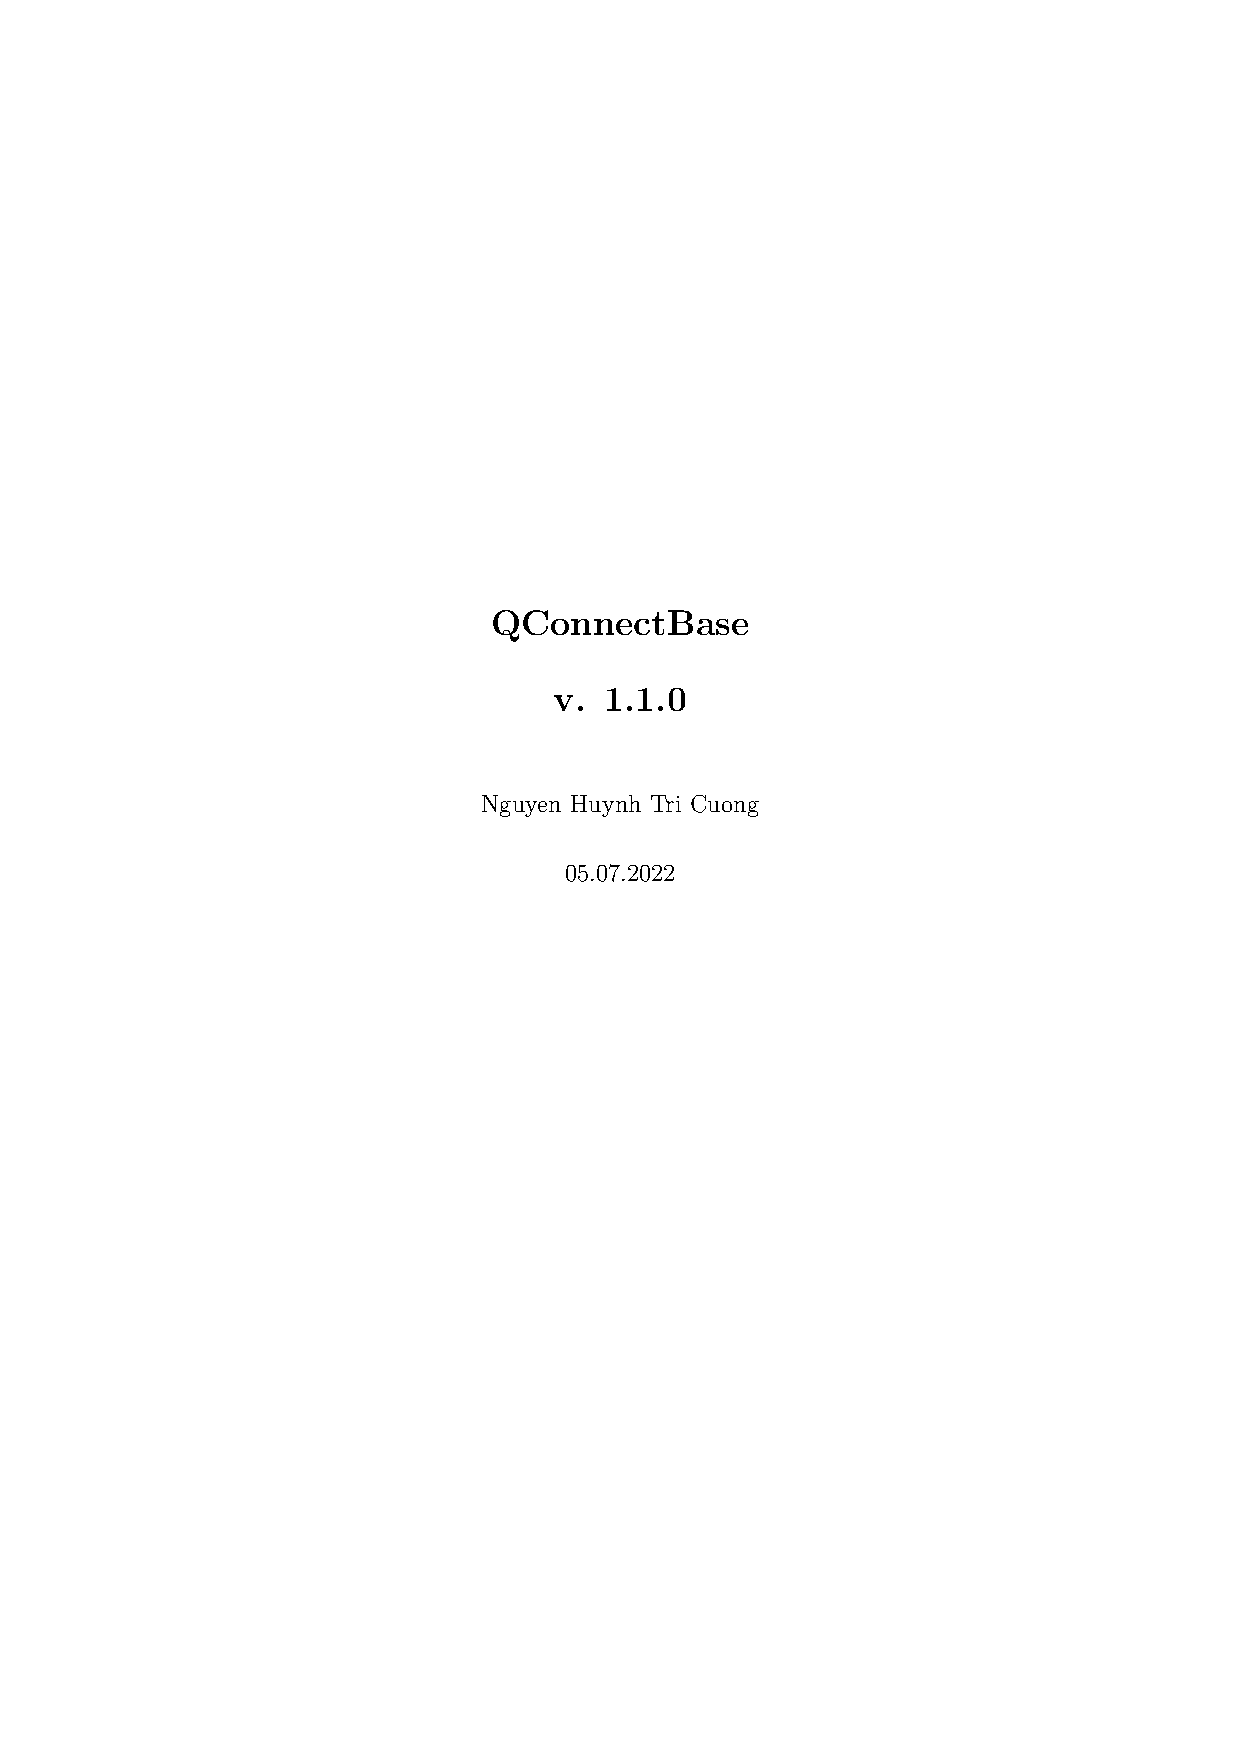
\includepdf[pages=1,pagecommand=\section{QConnectBase}]{./include/libraries/robotframework-qconnect-base/QConnectBase.pdf}
\includepdf[pages=2-,pagecommand={}]{./include/libraries/robotframework-qconnect-base/QConnectBase.pdf}
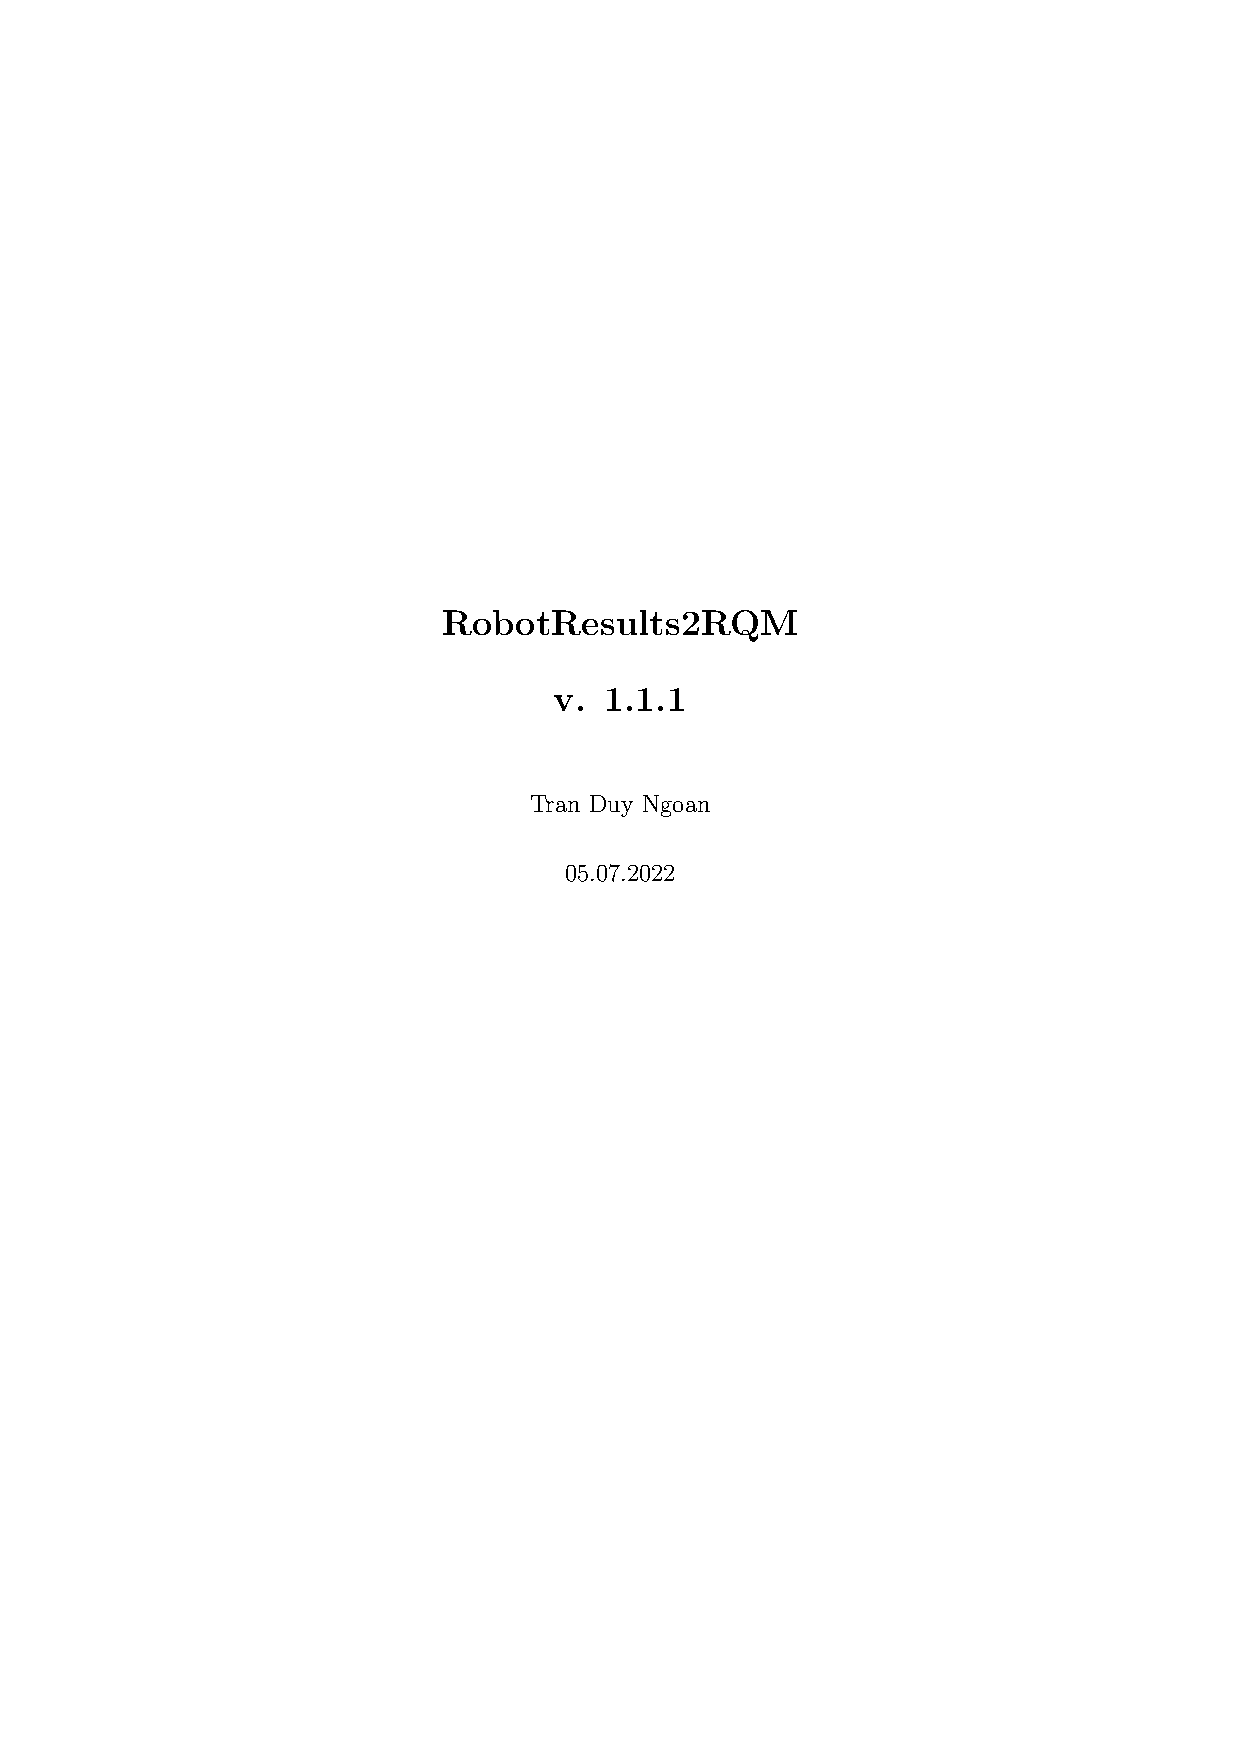
\includepdf[pages=1,pagecommand=\section{RobotResults2RQM}]{./include/libraries/robotframework-testresult2rqmtool/RobotResults2RQM.pdf}
\includepdf[pages=2-,pagecommand={}]{./include/libraries/robotframework-testresult2rqmtool/RobotResults2RQM.pdf}
\includepdf[pages=1,pagecommand=\section{RobotResults2DB}]{./include/libraries/robotframework-testresultwebapptool/RobotResults2DB.pdf}
\includepdf[pages=2-,pagecommand={}]{./include/libraries/robotframework-testresultwebapptool/RobotResults2DB.pdf}
\includepdf[pages=1,pagecommand=\section{TestResultWebApp}]{./include/libraries/testresultwebapp/TestResultWebApp.pdf}
\includepdf[pages=2-,pagecommand={}]{./include/libraries/testresultwebapp/TestResultWebApp.pdf}


\input{./externaldocs/final_summary}

% --------------------------------------------------------------------------------------------------------------
% appendix
% --------------------------------------------------------------------------------------------------------------

%\backmatter
%glossary and index would go here.

\end{document}
